\chapter{IMPLEMENTATION PLAN}

\section{Schedule (Gantt Chart)}

\begin{figure}[h]
\centering
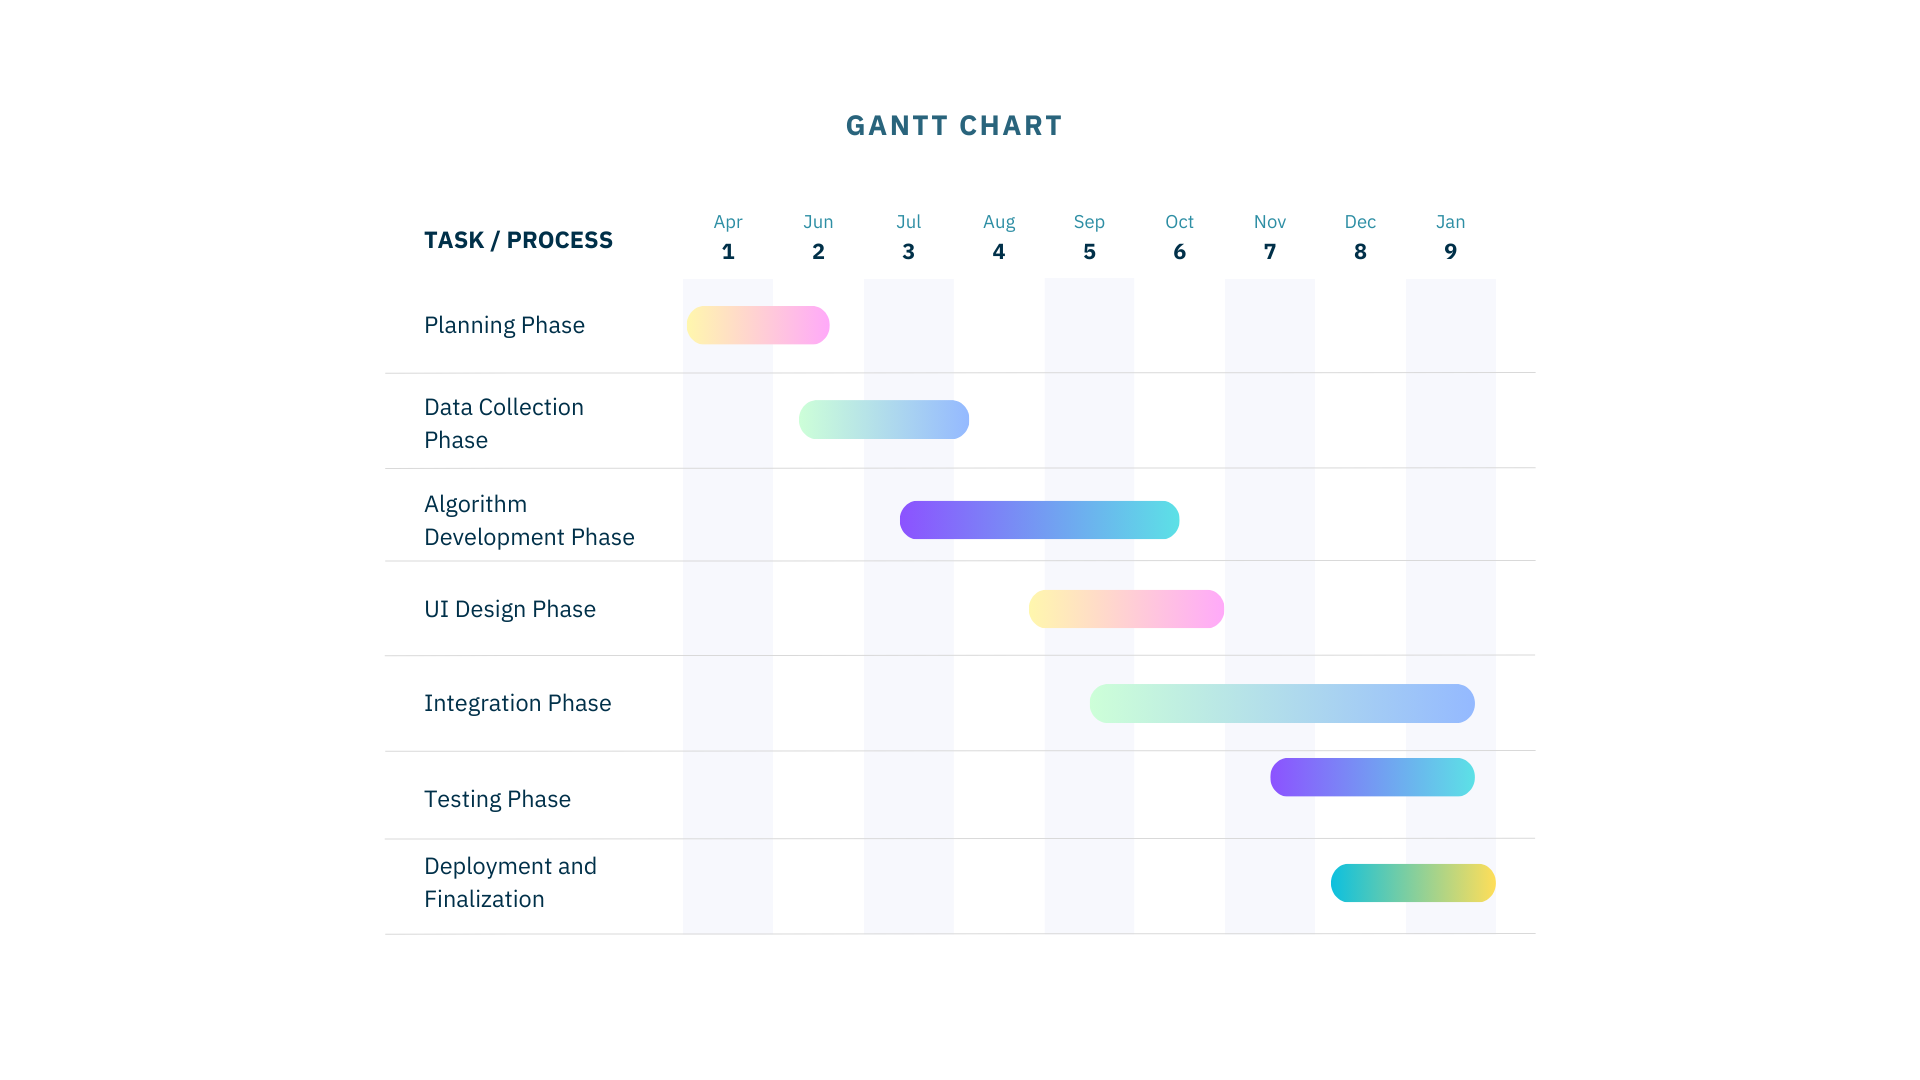
\includegraphics[width=1.0\textwidth]{./img/gantt_chart.png}
\caption{Gantt Chart}
\end{figure}

\section{Hardware and Software Requirements}

Our Tourist Recommendation System requires React.js, Tailwind CSS, FastAPI, Python, OpenCage, OpenStreetMap API keys, and VSCode, which are described below:

\subsection{Software Requirements}
Following are the software requirements for the project:

\subsubsection{Python}
Python is a high-level, interpreted programming language known for its simplicity, readability, and versatility. Python is the backbone for implementing machine learning algorithms, backend logic, and API services in this project.

\subsubsection{FastAPI}
FastAPI is a modern, fast web framework for building APIs with Python. It is used for creating the backend of the recommendation system, where it will handle requests, process user preferences, and return personalized attraction recommendations.

\subsubsection{OpenCage API}
OpenCage provides geocoding services, converting addresses into geographic coordinates (latitude, longitude) and vice versa. OpenCage's free API will be used to extract location data for map features and recommendations.

\subsubsection{OpenStreetMap API}
OpenStreetMap is an open-source mapping service. The OpenStreetMap API will be used for retrieving map data and visualizing tourist attractions for the user, enabling seamless navigation and recommendations.

\subsubsection{VS Code}
Visual Studio Code is a popular, open-source code editor that will be used for writing and editing all project code, supporting languages such as JavaScript, Python, and HTML/CSS.

\subsubsection{React.js}
React.js is a JavaScript library for building user interfaces, particularly for single-page applications. React allows developers to create reusable UI components, leading to more maintainable code. It will be used for the frontend of the Tourist Recommendation System.

\subsubsection{Tailwind CSS}
Tailwind CSS is a utility-first CSS framework that provides pre-defined classes for layout, styling, and responsive design. It allows developers to build modern user interfaces with minimal custom CSS, enabling rapid and consistent styling for the application.



\subsection{Hardware Requirements}
The hardware requirements for the project include:

\begin{itemize}
    \item A computer with sufficient RAM (8GB minimum) for development and testing.
    \item A reliable internet connection for API calls to OpenCage and OpenStreetMap.
    \item Access to cloud-based services (if necessary) for running the backend or storing large datasets.
    \item A development environment capable of running React.js, FastAPI, and Python applications.
\end{itemize}

\section{Cost Estimation}
The computational power costs for this project will primarily involve API usage for maps and geocoding services. The free API keys for OpenCage and OpenStreetMap will suffice for development and initial testing phases. However, as the system scales, there may be costs associated with higher API usage, server hosting, and potential cloud services if required for data storage or backend hosting.

\begin{itemize}
    \item OpenCage: The free tier allows up to 2,500 requests per day.
    \item OpenStreetMap: No direct costs for basic usage, but usage may be limited for high-traffic applications.
    \item Server Hosting: A cost for hosting the backend API, which could be minimal for initial testing (e.g., using services like Heroku or Vercel for free).
\end{itemize}

Regular monitoring and optimization will be necessary to keep resource consumption and costs manageable. Free-tier API services will help minimize costs during early stages, but as the system grows, paid services might be required.

